\section{ForenX-Bench Evaluation Set-up}
\FloatBarrier

\subsection{Datasets and annotation scope}
We evaluated three existing image-manipulation datasets without redistributing their source files. Columbia Uncompressed contributes 363 images (183 authentic and 180 spliced). The provided blue-region annotation is specific to the dataset's splice-boundary/camera-region convention and is not treated as a general complete tampered-area mask. Corrected CASIA v1 contributes 1,721 images (800 authentic and 921 tampered); 920 tampered images have dimension-aligned pixel masks. Corrected COVERAGE contributes 200 images in 100 authentic--tampered pairs; 91 tampered images have masks dimensionally aligned with their image. All 200 COVERAGE images are retained for detection, while the nine mismatched masks are excluded only from localization. The dataset sources and annotation denominators are summarized in Table~\ref{tab:datasets}.

\begin{table}[t]
\centering
\caption{Evaluation data and valid annotation scope. Counts refer to the corrected local dataset bundles used in this study. Columbia reference annotations have dataset-specific semantics and must not be interpreted as complete manipulation masks.}
\label{tab:datasets}
\small
\resizebox{\textwidth}{!}{%
\begin{tabular}{lrrrrl}
\toprule
Dataset & Authentic & Manipulated & Detection $n$ & Valid masks & Manipulation type \\
\midrule
Columbia Uncompressed & 183 & 180 & 363 & 180$^*$ & Splicing \\
CASIA v1 corrected & 800 & 921 & 1,721 & 920 & Splicing, copy-move \\
COVERAGE corrected & 100 & 100 & 200 & 91 & Copy-move \\
\bottomrule
\end{tabular}
}
\\[0.25em]
\parbox{\linewidth}{\footnotesize $^*$The Columbia reference has splice-boundary/camera-region semantics, so its pixel metrics are reported separately and are not directly comparable to complete manipulated-region masks.}
\end{table}

\subsection{Sample integrity and provenance}
Each evaluated input is identified by a dataset-relative sample identifier and a SHA-256 digest. Dataset manifests record the source bundle, class label, manipulation category where available, dimensions, mask availability and integrity information. Model outputs and stress derivatives are linked to the originating image through records that identify the model artifact and transformation parameters. The raw datasets and model weights remain outside the project archive; acquisition instructions and checksums support users in obtaining and validating their own copies under the upstream conditions.

\begin{figure}[t]
\centering
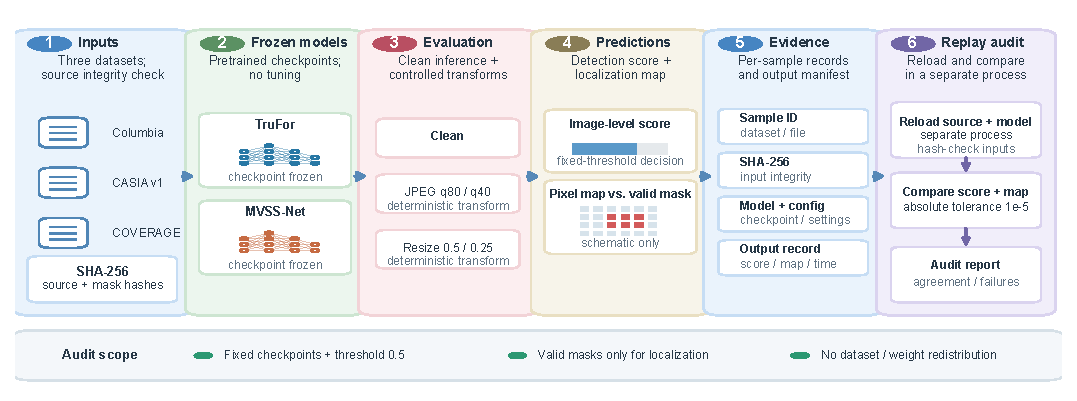
\includegraphics[width=\linewidth]{reports/figures/evaluation_workflow.pdf}
\caption{ForenX-Bench evaluation and audit workflow. Dataset files are integrity-checked before inference with frozen TruFor and MVSS-Net checkpoints. Clean and controlled transformed inputs are evaluated for image-level detection and mask-based localization where reference masks are valid. Sample-level records retain input identity, hashes, model/configuration information and outputs. A stratified subset is reprocessed independently and compared with stored outputs at an absolute tolerance of $10^{-5}$. The map and mask icons are schematic; datasets and model weights are not redistributed.}
\label{fig:workflow}
\end{figure}

\FloatBarrier
\subsection{Frozen model artifacts}
The evaluation uses released TruFor and MVSS-Net implementations and checkpoints without additional training or threshold tuning on the evaluation datasets \cite{guillaro2023trufor,chen2021mvss}. TruFor was executed at upstream code commit \texttt{ae54475d\allowbreak{}f6f41a49\allowbreak{}1d761510\allowbreak{}0feb1926\allowbreak{}3dec13f7}; the checkpoint MD5 recorded in the experiment provenance is \texttt{7bee48f3\allowbreak{}476c7561\allowbreak{}6c3c5721\allowbreak{}ab256ff8}. MVSS-Net used the authors' CASIAv2 checkpoint, recorded by SHA-256 \texttt{080bc6c3\allowbreak{}aae59f74\allowbreak{}8b547dbf\allowbreak{}090786fe\allowbreak{}9d31a6e5\allowbreak{}0749daaa\allowbreak{}40871e29\allowbreak{}8d6a7e50}. Both image-level and pixel-map decisions use a fixed threshold of 0.5. Since MVSS-Net was trained with CASIAv2 data and the locally reconstructed CASIA v1 set is not the official CASIAv1plus construction, potential source overlap limits interpretation of its CASIA result as fully independent.

\subsection{Controlled digital stress transformations}
For Columbia and CASIA v1, each original image was processed under four deterministic conditions: JPEG recompression at quality 80, JPEG recompression at quality 40, resize to 0.5 times followed by restoration to the original dimensions, and resize to 0.25 times followed by restoration. Transformation manifests preserve the condition and source-image link. These conditions probe sensitivity to compression and resolution loss; they do not model a named social platform, physical screen recapture, or every real-world processing chain. COVERAGE is used for clean-image detection and valid-mask localization in the current release, without the same four-condition pressure-test suite.

\subsection{Evidence records}
For every CASIA v1 image--model pair, the workflow writes one JSONL evidence record. Required fields include the bounded image-level prediction claim, image and output identifiers, source hash, frozen model identity, operation/configuration reference, output-file integrity data, and applicability and failure notes. This record is an auditable computational trace; it is not a human-authored forensic opinion and does not assert that a model cue uniquely identifies manipulation.
